\documentclass{article} % For LaTeX2e
\usepackage{nips13submit_e,times}
\usepackage{amsmath}
\usepackage{amssymb}
\usepackage{comment}
\usepackage{hyperref}
\usepackage{enumerate}
\usepackage{enumitem}
\usepackage{cleveref}
\usepackage{graphicx}
\usepackage{url}
\usepackage{placeins}
\usepackage{fancyvrb}
\usepackage[font={small,it},width=5in]{caption}
%\documentstyle[nips13submit_09,times,art10]{article} % For LaTeX 2.09


\title{Musical Structure in Irish Traditional Tunes}

\author{Matthew Staib, Lennart Jansson, and Edward Dai}

\newcommand{\fix}{\marginpar{FIX}}
\newcommand{\new}{\marginpar{NEW}}

\newcommand{\xip}{x^{(i)}}
\newcommand{\xjp}{x^{(j)}}
\newcommand{\xkp}{x^{(k)}}
\newcommand{\yip}{y^{(i)}}
\newcommand{\yjp}{y^{(j)}}
\newcommand{\ykp}{y^{(k)}}
\newcommand{\vectornorm}[1]{\left\| #1 \right\|}

\nipsfinalcopy % Uncomment for camera-ready version

\begin{document}
\suppressfloats
\maketitle

\section{Introduction}
Most Irish traditional folk dance music contains two musical themes; the tune
begins with one musical theme which is usually repeated, then progresses to
another theme with similar musical structure and motives, which is usually also
repeated. The first section is typically called the $A$ section while the second
is called the $B$ section. Our goal is to understand, at a quantitative level,
the musical relationship between $A$ sections and $B$ sections. See
\cref{origtune} for an example.

In working towards this goal, we need to understand both the relationship
between the $A$ and $B$ sections of a given folk song as well as the differences
between $A$ and $B$ sections of the tunes in general. In the long term we wish
to, given an $A$ section, automatically generate a musically appropriate $B$
section.

\begin{figure}
  \centering 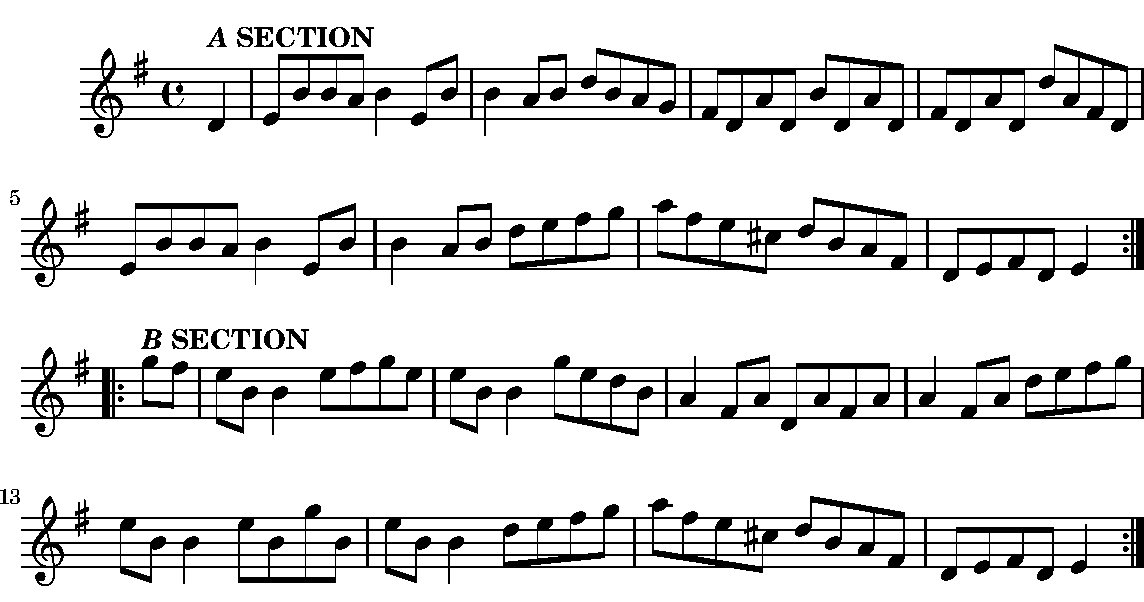
\includegraphics[width=4in]{original_tune-crop.pdf}
  \caption{
    ``Cooley's (reel)'', an example of a traditional Irish tune from The
    Session \cite{thesession}. This reel has the standard form of an 8-bar $A$
    section which is repeated, then an 8-bar $B$ section which is also repeated.
    The sections are labeled in the notation above. Notice how the $A$ and $B$
    sections contain distinct melodic lines, but still have musical similarity.
    For example, they end with the same $2 \frac 1 2$ bar
    ascending-then-descending motif.
  }
  \label{origtune}
\end{figure}

\section{Dataset}

We are using the tunes dataset from The Session \cite{thesession}. The
Session is an online community of people who are interested in playing Irish
folk music and cataloguing traditional Irish tunes for others to learn. These
tunes include various dance forms, such as jigs, reels, waltzes, and slides.
Available on their website is a set of roughly 21,000 dance tune settings
in ABC notation, a human-readable symbolic music data format in plain text. The
ABC files are easily parsed and manipulated symbolically for feature extraction.

\section{Feature Extraction}

First we select from our dataset tunes which have the standard form of an $A$
and a $B$ section. We consider only tunes with a number of bars in $\{16, 32,
64\}$: an individual $A$ or $B$ section usually has 8 or 16 measures, or 16 or
32 after manually reduplicating out music that was contained in repeat signs. We
want to restrict to tunes that split evenly into two sections (e.g.  not three
sections, which could mean $ABC$, $ABA$, etc.).

After splitting tunes into $A$ and $B$ sections, we turn our attention to
feature extraction.  Our dataset is loosely in the form of sequences of pitches
representing melodies. However, as tunes may have different lengths, we need to
generate a feature vector of fixed length.

We define an $n$-gram as an ordered list of (in our case) $n$ pitches of notes
in a melody, ignoring accidentals. In total, we created three different feature
vector designs.
\begin{enumerate}
%TODO: consider using nouns instead of verbs.
\item Record counts of all 1- and 2-grams.

\item Split melodies by measure into eighths and store counts of all 1- and
2-grams separately for each measure.

\item Use the features from (2), also adding counts of notes of particular
  rhythmic length.
\end{enumerate}

Since these feature vectors have nearly 2,000 components, before further
processing, we used PCA to reduce the number of components. This 
helped make metric learning computationally more feasible.

\section{SVM Classifier}
Using our labeled pool of $A$ and $B$ sections, we used an SVM with Gaussian
kernel to attempt to classify a given segment of a tune as an $A$ section or a
$B$ section. We used 8-fold cross-validation, and experimented with our three
different feature vectors and various numbers of PCA components. To train the
SVM, we used the relevant Scikit-learn libraries \cite{sklearn}.

\begin{figure}
  \centering 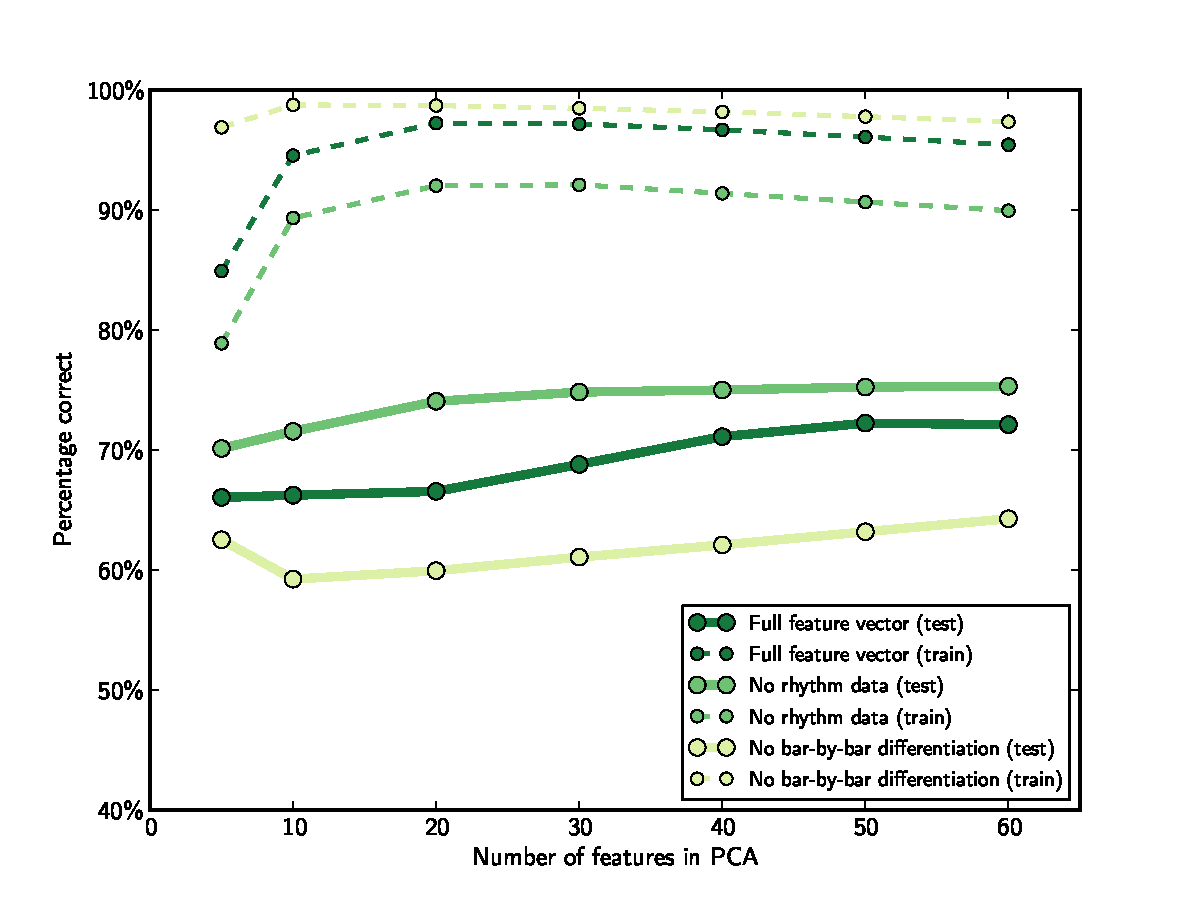
\includegraphics[width=4in]{../svm_results/svm.pdf}
  \caption{
    Accuracy of running our SVM classifier to classify musical phrases as either
    $A$ or $B$ sections. The performance on the testing dataset with various
    feature vector designs is shown with solid lines, and the performance on the
    original training set is shown in dotted lines.
  }
  \label{svmfig}
\end{figure}

Our SVM classification results are presented in \cref{svmfig}. For all three
feature vector designs, performance on the test set generally improved when we
kept a greater number of features when running PCA on the data. Accuracy on
the training sets was much better than the testing sets---probably, this is due
to overfitting the SVM to the particular training sets in each case. 

The feature vector design that gave us the least difference between training and
testing performance (so probably represents the feature vector design with the
least overfitting) is the ``no rhythm data'' feature vector, that contains
pitch $n$-gram counts specific to each bar of the tune but not overall counts of
notes with particular rhythmic values. Interestingly, the full feature vector
with rhythm information caused the SVM classifier to perform worse. We believe
this is because the corresponding $A$ and $B$ sections of most tunes may have
different melodic figures, but if they are to have reasonable stylistic
similarity they are likely to have similar rhythm value counts (for example, a
reel whose $A$ section is mostly eighth notes is likely to have a $B$ section
which contains mostly eighth notes). Meanwhile, having bar-by-bar
differentiation of features understandably greatly improved performance---we
believe this is a consequence of how in many tunes, the last bars of the $A$ and
$B$ sections contain nearly the same notes. Thus our SVM might have learned to
give greater weighting to the musical features of earlier bars, which are likely
to be distinctive to $A$ and $B$ sections.

%Observe that when
%we use the more complex feature vectors, training performance improves, but test
%performance suffers. We attribute this to overfitting; namely, as our feature
%vectors become more descriptive, the SVM identifies particular patterns present
%only in the training data.

\section{Metric Learning Problem Formulation}
We also want to learn what makes the $A$ and $B$ sections of a particular tune
musically related. We attempt to learn a metric $d(x, y)$ where, if $x, y \in
\mathbb{R}^n$ are the feature vectors corresponding to the $A$ and $B$ sections
of a tune, $d(x, y)$ should be small. For this task, we use the Mahalanobis
metric, given by
\[
d(x,y) = \vectornorm{x-y}_M = \sqrt{(x-y)^T M (x-y)}
\] 
for $M \in \mathbb{R}^{n\times n}$ positive semidefinite, and attempt to learn a
suitable value of $M$.

Usually, in metric learning, one learns a metric by supplying both pairs of
points $(\xip, \xjp) \in \mathcal{S}$ that are similar and should have small
distance, and points $(\yip, \yjp) \in \mathcal{D}$ that are dissimilar and
should have large distance. We then solve the following optimization problem for
$M$ (from \cite{metricNg}):
\begin{align*} 
\text{minimize: } &
\sum_{(x^{(i)}, x^{(j)}) \in \mathcal S} \vectornorm{x^{(i)} - x^{(j)}}_M^2 \\
\text{subject to: }
& \sum_{(y^{(i)}, y^{(j)}) \in \mathcal D}
	\vectornorm{y^{(i)} - y^{(j)}}_M^2 \ge 1, \\
& M \succeq 0.
\end{align*} 
However, in our problem, it is unclear how to select pairs of $A$ and $B$
sections that are dissimilar. Intuitively, one might argue that the $A$ and $B$
sections of different tunes should be dissimilar. However, two arbitrary tunes
may be variations of each other, and hence have $A$ and $B$ sections that are
related.

Note that by simply removing the dissimilarity constraint results in an
optimization problem whose optimal value $M$ is the zero matrix. Instead, we
enforce $\det M = 1$ as a reasonable-seeming regularity constraint. We do this
by noting that $\det M$ is concave and so 
$(\det M)^{1/n} \ge 1 \Leftrightarrow \det M \geq 1$ is a
convex constraint \cite{boyd}. Then, the optimization problem,

\begin{align*} 
\text{minimize: } & \sum_{k=1}^m \vectornorm{x^{(k)} - y^{(k)}}_M^2 \\
\text{subject to: }
& M \succeq 0, \\
& (\det M)^{1/n} \ge 1,
\end{align*} 
where $m$ is the number of training examples, produces $M$ with $\det M = 1$, as
the objective function scales with the determinant of $M$.

\section{Metric Learning Implementation and Results}
\begin{figure}
  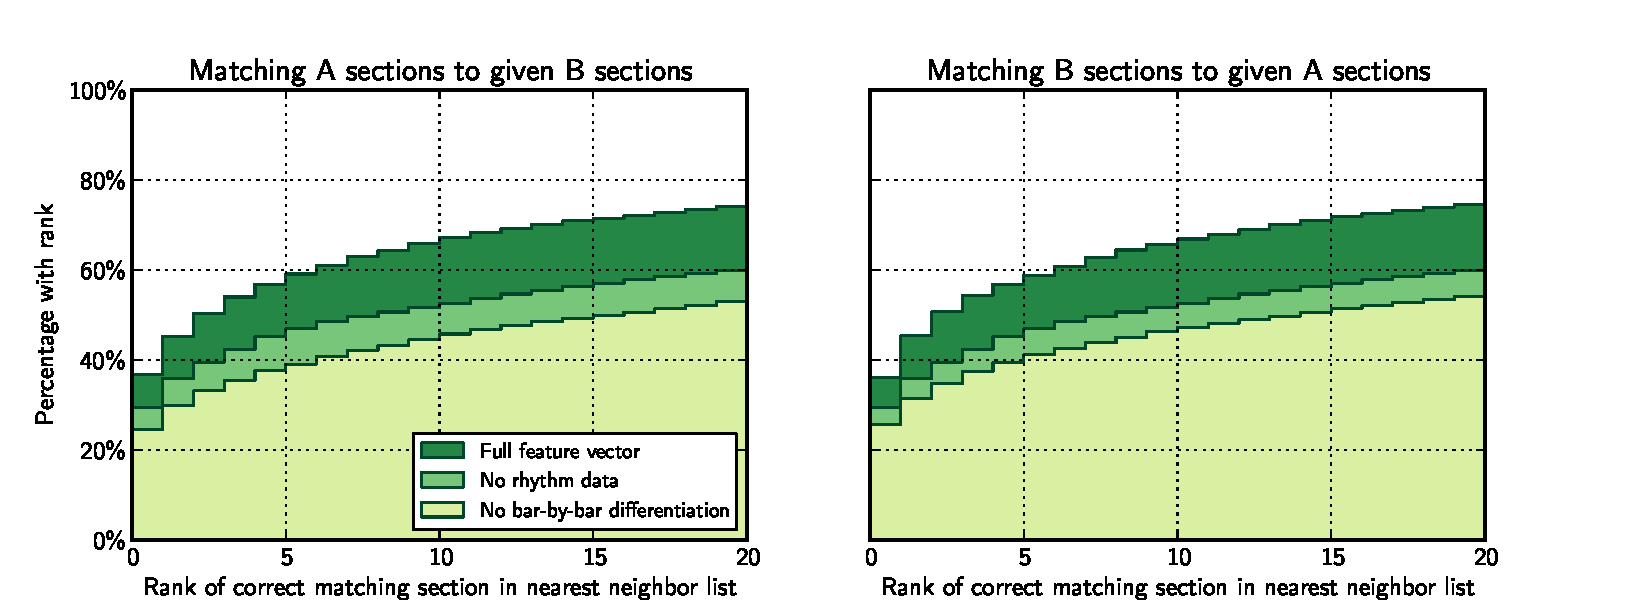
\includegraphics[width=5.8in]{../trial_data_logs/hists.pdf}
  \caption{
    Results of metric learning-based matching algorithm, showing the percentage
    of tune sections whose matching other section appeared at a given rank in a
    ranked list of nearest neighbors by the learned metric. For example, the
    first column in the left chart represents the percentage of $B$ sections
    whose matching $A$ section was the very closest by the metric out of all
    possible other $A$ sections. Here the full feature vector with rhythm
    information gave by far the best performance.
  }
  \label{hists}
\end{figure}

After using PCA to reduce our feature vectors to $n = 35$ components, we applied
this method using 8-fold cross-validation to learn such a metric $d$. We used
CVX to solve the optimization problem that determines $M$ \cite{cvx}.
To evaluate the success of our metric, we consider the following problem:
\begin{itemize}
\item[] Split apart the $A$ and $B$ sections of our test data ($\approx 1000$
tunes). For each $A$ section, order all the $B$ sections by increasing distance
from this $A$ section (under the metric $d$). Record the rank in this list of
the actual corresponding $B$ section. Ideally, the actual $B$ section would be
the first element of this list, closest to this $A$ section. Alternatively, we
could match an $A$ section to a given $B$ section.
\end{itemize}
%We made a cumulative histogram of the ranks of the actual sections.%TODO: See Figure
%We also broke down the frequency of these ranks into a pie chart. %TODO: Fig
See \cref{hists} for a cumulative histogram of our results.
If we were to randomly guess the closest $B$ section, we would expect the rank
of the correct $B$ section to be 1 with probability 0.1\%. In our results, the
correct $B$ section was the first ranking option 37\% of the time. Moreover, the
correct $B$ section was in the top 10\% of the ranking 93\% of the time. We
conclude that there is a significant amount of information shared between $A$
sections and $B$ sections, and the Mahalanobis metric we learned is able to
identify some of the musical similarities.
%TODO: caption and labels and resize

\section{Composition}
Now that we have shown the viability of our metric, we can use it to try to,
given an $A$ section, compose a musically related $B$ section. We employed a
simple algorithm:
\begin{enumerate}
\item Select a specific tune, and split it into its $A$ and $B$ sections.

\item Randomize a $B$ section ($b_{cur}$) using the rhythm of the $A$ section.

\item Repeat $n$ times:
\begin{itemize}\parskip=0.05in
\item[] For every $i \in \{1, \dots, k\}$:
\begin{itemize}
\item[] Generate $b_i$ by randomly making pitch edits to $b_{cur}$.
\end{itemize}
\item[] Set
$\displaystyle{b_{cur} := \arg \min_{b_i} \  d(b_i, A)}$.
\end{itemize}
\end{enumerate}
As an example, we tried to compose a new $B$ section for the $A$ section of
Cooley's reel, the original correct version of which can be seen in
\cref{origtune}. Our new created $B$ section can be seen in \cref{newb}. %TODO
\begin{figure}
  \centering
  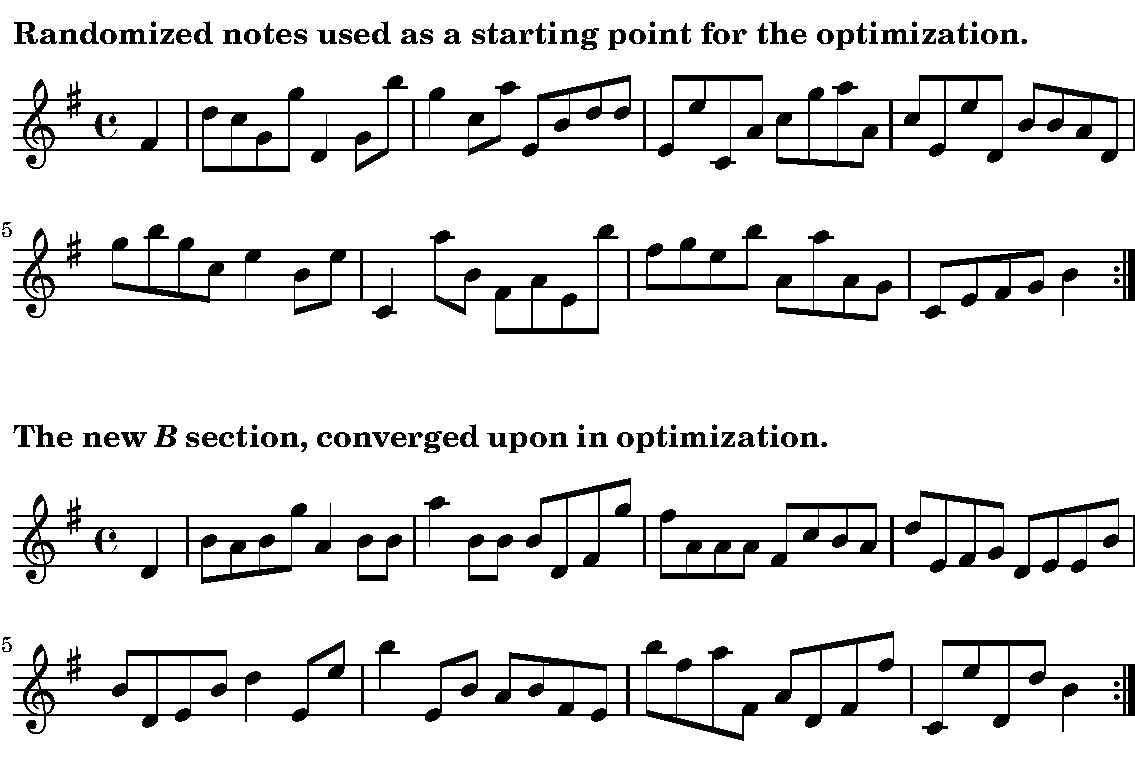
\includegraphics[width=4in]{new_b-crop.pdf}
  \caption{
    A new $B$ section composed for Cooley's (see \cref{origtune}), using its distance
    by the learned metric to the original $A$ section.
  }
  \label{newb}
\end{figure}

While the resulting $B$ section is musically far from ideal, it is notably
better than the random starting $B$ section. For example, the starting note is
the same as that of the tune and the intervals between consecutive notes are, on
average, smaller.

\section{Further Work}
At a broad level, all the work we have done could be improved by better feature
selection. Given the complexities of music, 1- and 2-grams are far from ideal
features. At the very least, we could store counts of 3- or 4- (or more) grams,
or subsets of these, thus encapsulating more of what a melody looks like on a
larger scale. There are other obvious musical features that we have not looked
into using, for example, time and key signatures. Even more musically-complex
features may prove fruitful, for example, based on the notes in the melody at
each point in time we could infer the chord progression. There is a lot left
to explore in this regard.

As for improvements specific to our automated composition, one idea is to
use our dataset to construct a model for the likelihood that a given sequence
of pitches is musically significant. At the moment we are easily able to
``converge'' to a $B$ section that, with respect to our learned metric, is
actually closer to the given $A$ section than the actual $B$ section of the
tune is. We produce a sequence of pitches that is similar to the $A$ section
but that, when viewed independently of this $A$ section, still seems musically
``unlikely.'' It is does not seem unreasonable, for example, that we could
learn from our set of tunes that smaller intervals between notes are much more
likely than large ones. One other complicating issue is that when performing PCA
to reduce our feature vectors to only have at most 35 features (as is necessary
for the metric learning implementation), we may lose essential musical
information that is necessary for a tune to seem plausible to a human, as
features that are unrelated musically may be represented by a single
principal component in the transformed dataset. We might find improvements to
the composition process by using a metric or likelihood estimation that is able
to consider a larger number of features, or perhaps the untransformed original
feature vectors themselves.

%In short, while we believe we have made significant progress, there is no
%shortage of future work to be done.

%I gave up. We're using this instead of the BibTex database. (ED)
%Format is "\bibitem{cite_key} bibliographic information ...."
%Cite using \cite{cite_key}.
%Make sure that these are all used and look decent.
\begin{thebibliography}{9}

\bibitem{boyd}
S. Boyd and L. Vandenberghe, \textit{Convex Optimization}, Cambridge University
Press, 2004.

\bibitem{cvx}
M. Grant and S. Boyd. CVX: Matlab software for disciplined convex
programming, version 2.0 beta. \texttt{http://cvxr.com/cvx}, September 2013.

\bibitem{sklearn}
F. Pedregosa et al. Scikit-learn: Machine learning in Python. 
\textit{Journal of Machine Learning Research}, \textbf{12}, 2825-2830.

\bibitem{thesession} 
The Session (\texttt{thesession.org}).

\bibitem{metricNg} 
E. Xing, A. Ng, M. Jordan, and S. Russell. Distance Metric Learning, with
Application to Clustering with Side-Information. \textit{NIPS}. 2002.

\end{thebibliography}

\end{document}
